%% This is an example first chapter.  You should put chapter/appendix that you
%% write into a separate file, and add a line \include{yourfilename} to
%% main.tex, where `yourfilename.tex' is the name of the chapter/appendix file.
%% You can process specific files by typing their names in at the 
%% \files=
%% prompt when you run the file main.tex through LaTeX.

\singlespacing{

\chapter{Implementation}\label{chap:implementation}

Anisotropic Modeling of Engineered Bits and Atoms (\href{http://git.amandaghassaei.com/AMOEBA/}{AMOEBA}), is a 3D CAD and simulation tool, based off the ideas from Chapters \ref{chap:CAD} and \ref{chap:functionSim}.  In this tool, users construct assemblies of functional primitives and simulate their electronic and mechanical behaviors.  It is available to demo \href{http://git.amandaghassaei.com/AMOEBA/}{online} and the source code can be found on \href{https://github.com/amandaghassaei/AMOEBA}{Github}.  AMOEBA primarily serves as a research tool for quickly simulating assemblies of functional digital material parts that we are developing in the lab.  However, it's a very flexible platform, and I'm curious to see what other people might use it for.  When it's in a more stable state I will write up some documentation and push it out to a wider audience.  This chapter introduces information about the software implementation of AMOEBA.

\section{Javascript/WebGL}

AMOEBA was written in HTML5/JavaScript and currently hosted online.  I chose the web as a development platform for this project because it allows easier access to the code than any other platform.  Though user studies are not a component of this work, there is a long history of communities of users building things in sandbox environments that surpass anything the developers were able to imagine.  There is a lot of talent beyond the immediate neighborhood of CBA, and I'd like to try to make this codebase accessible to anyone interested in exploring the design space around digital materials.\\

The web app was written with the following dependencies:
\begin{itemize}
\setlength\itemsep{0em}
\item \href{http://threejs.org/}{Three.js} is a library containing lots of useful classes for interacting with WebGL without getting bogged down in the details or sacrificing too much in performance.
\item \href{http://requirejs.org/}{RequireJS} is a framework for asynchronously loading JavaScript modules and dependencies.
\item \href{http://backbonejs.org/}{Backbone.js} is a framework for managing UI events and giving structure to complex, interactive applications.
\item \href{https://jquery.com/}{JQuery} is a library that handles interactions between HTML and Javascript and helps maintain cross browser support of UI elements.
\item \href{http://underscorejs.org/}{Underscore} is a library with lots of useful functions for dealing with arrays and JavaScript objects.  Underscore also provides templating for Backbone.
\end{itemize}

\begin{figure}
  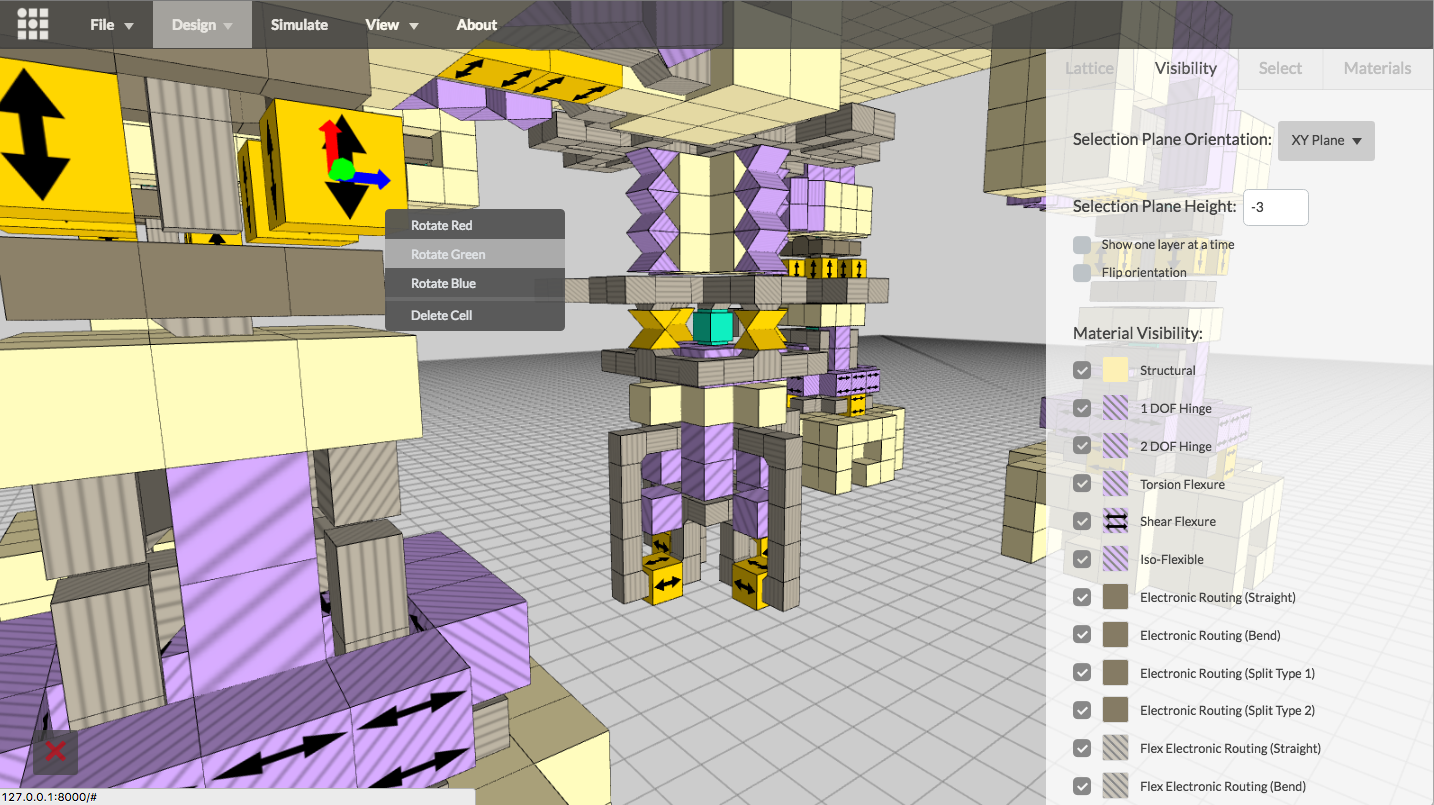
\includegraphics[width=\linewidth]{rotationGUI.png}
  \caption{A schematic diagram of a robotic ``pick and place'' in AMOEBA.  Cell rotation GUI allows anisotropic cells to be oriented in any direction.}
  \label{fig:rotationGUI}
\end{figure}

\begin{figure}
  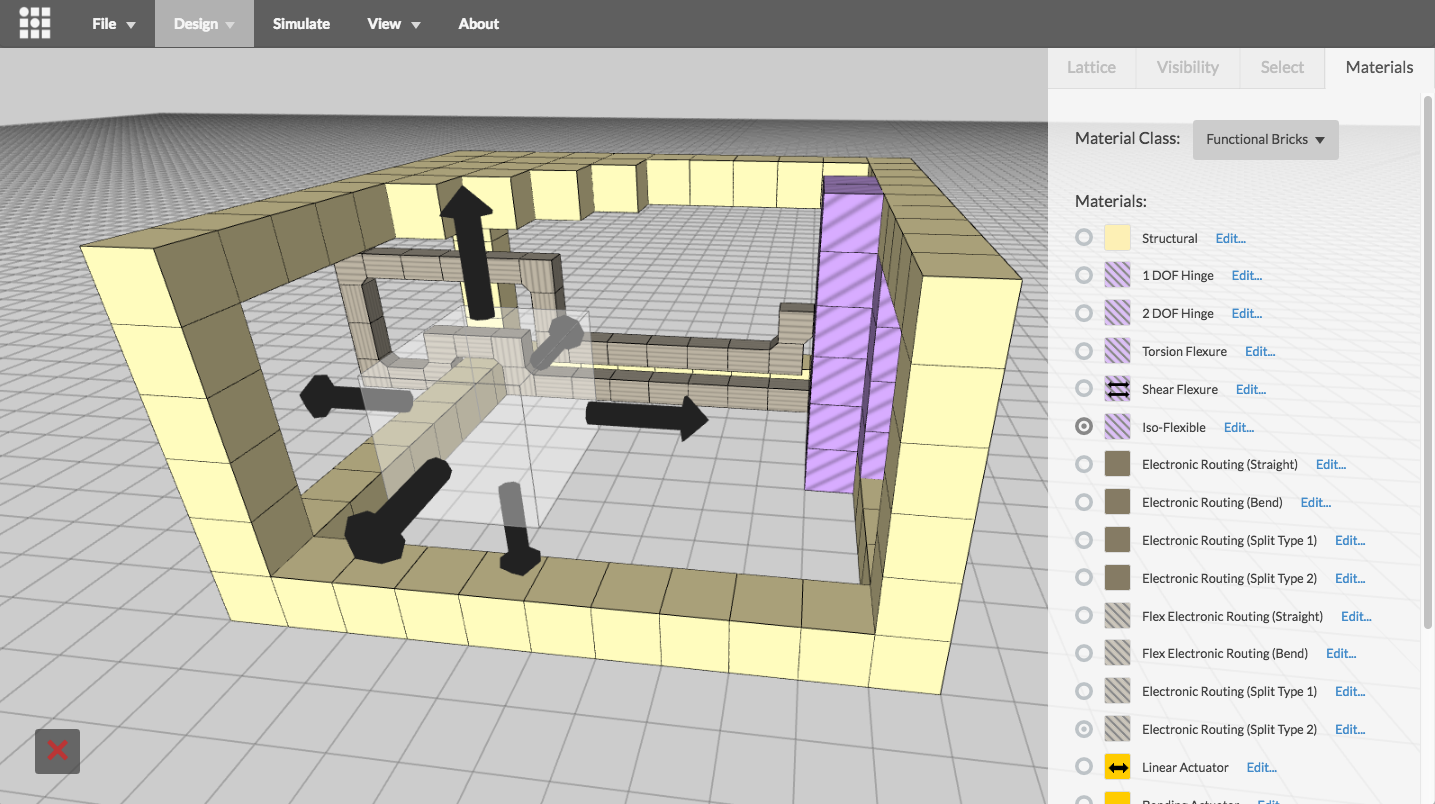
\includegraphics[width=\linewidth]{selectiontoolGUI.png}
  \caption{3D selection tool allows for bulk cell additions and removals, and cloning or mirroring existing geometry.}
  \label{fig:selectiontoolGUI}
\end{figure}

\begin{figure}
  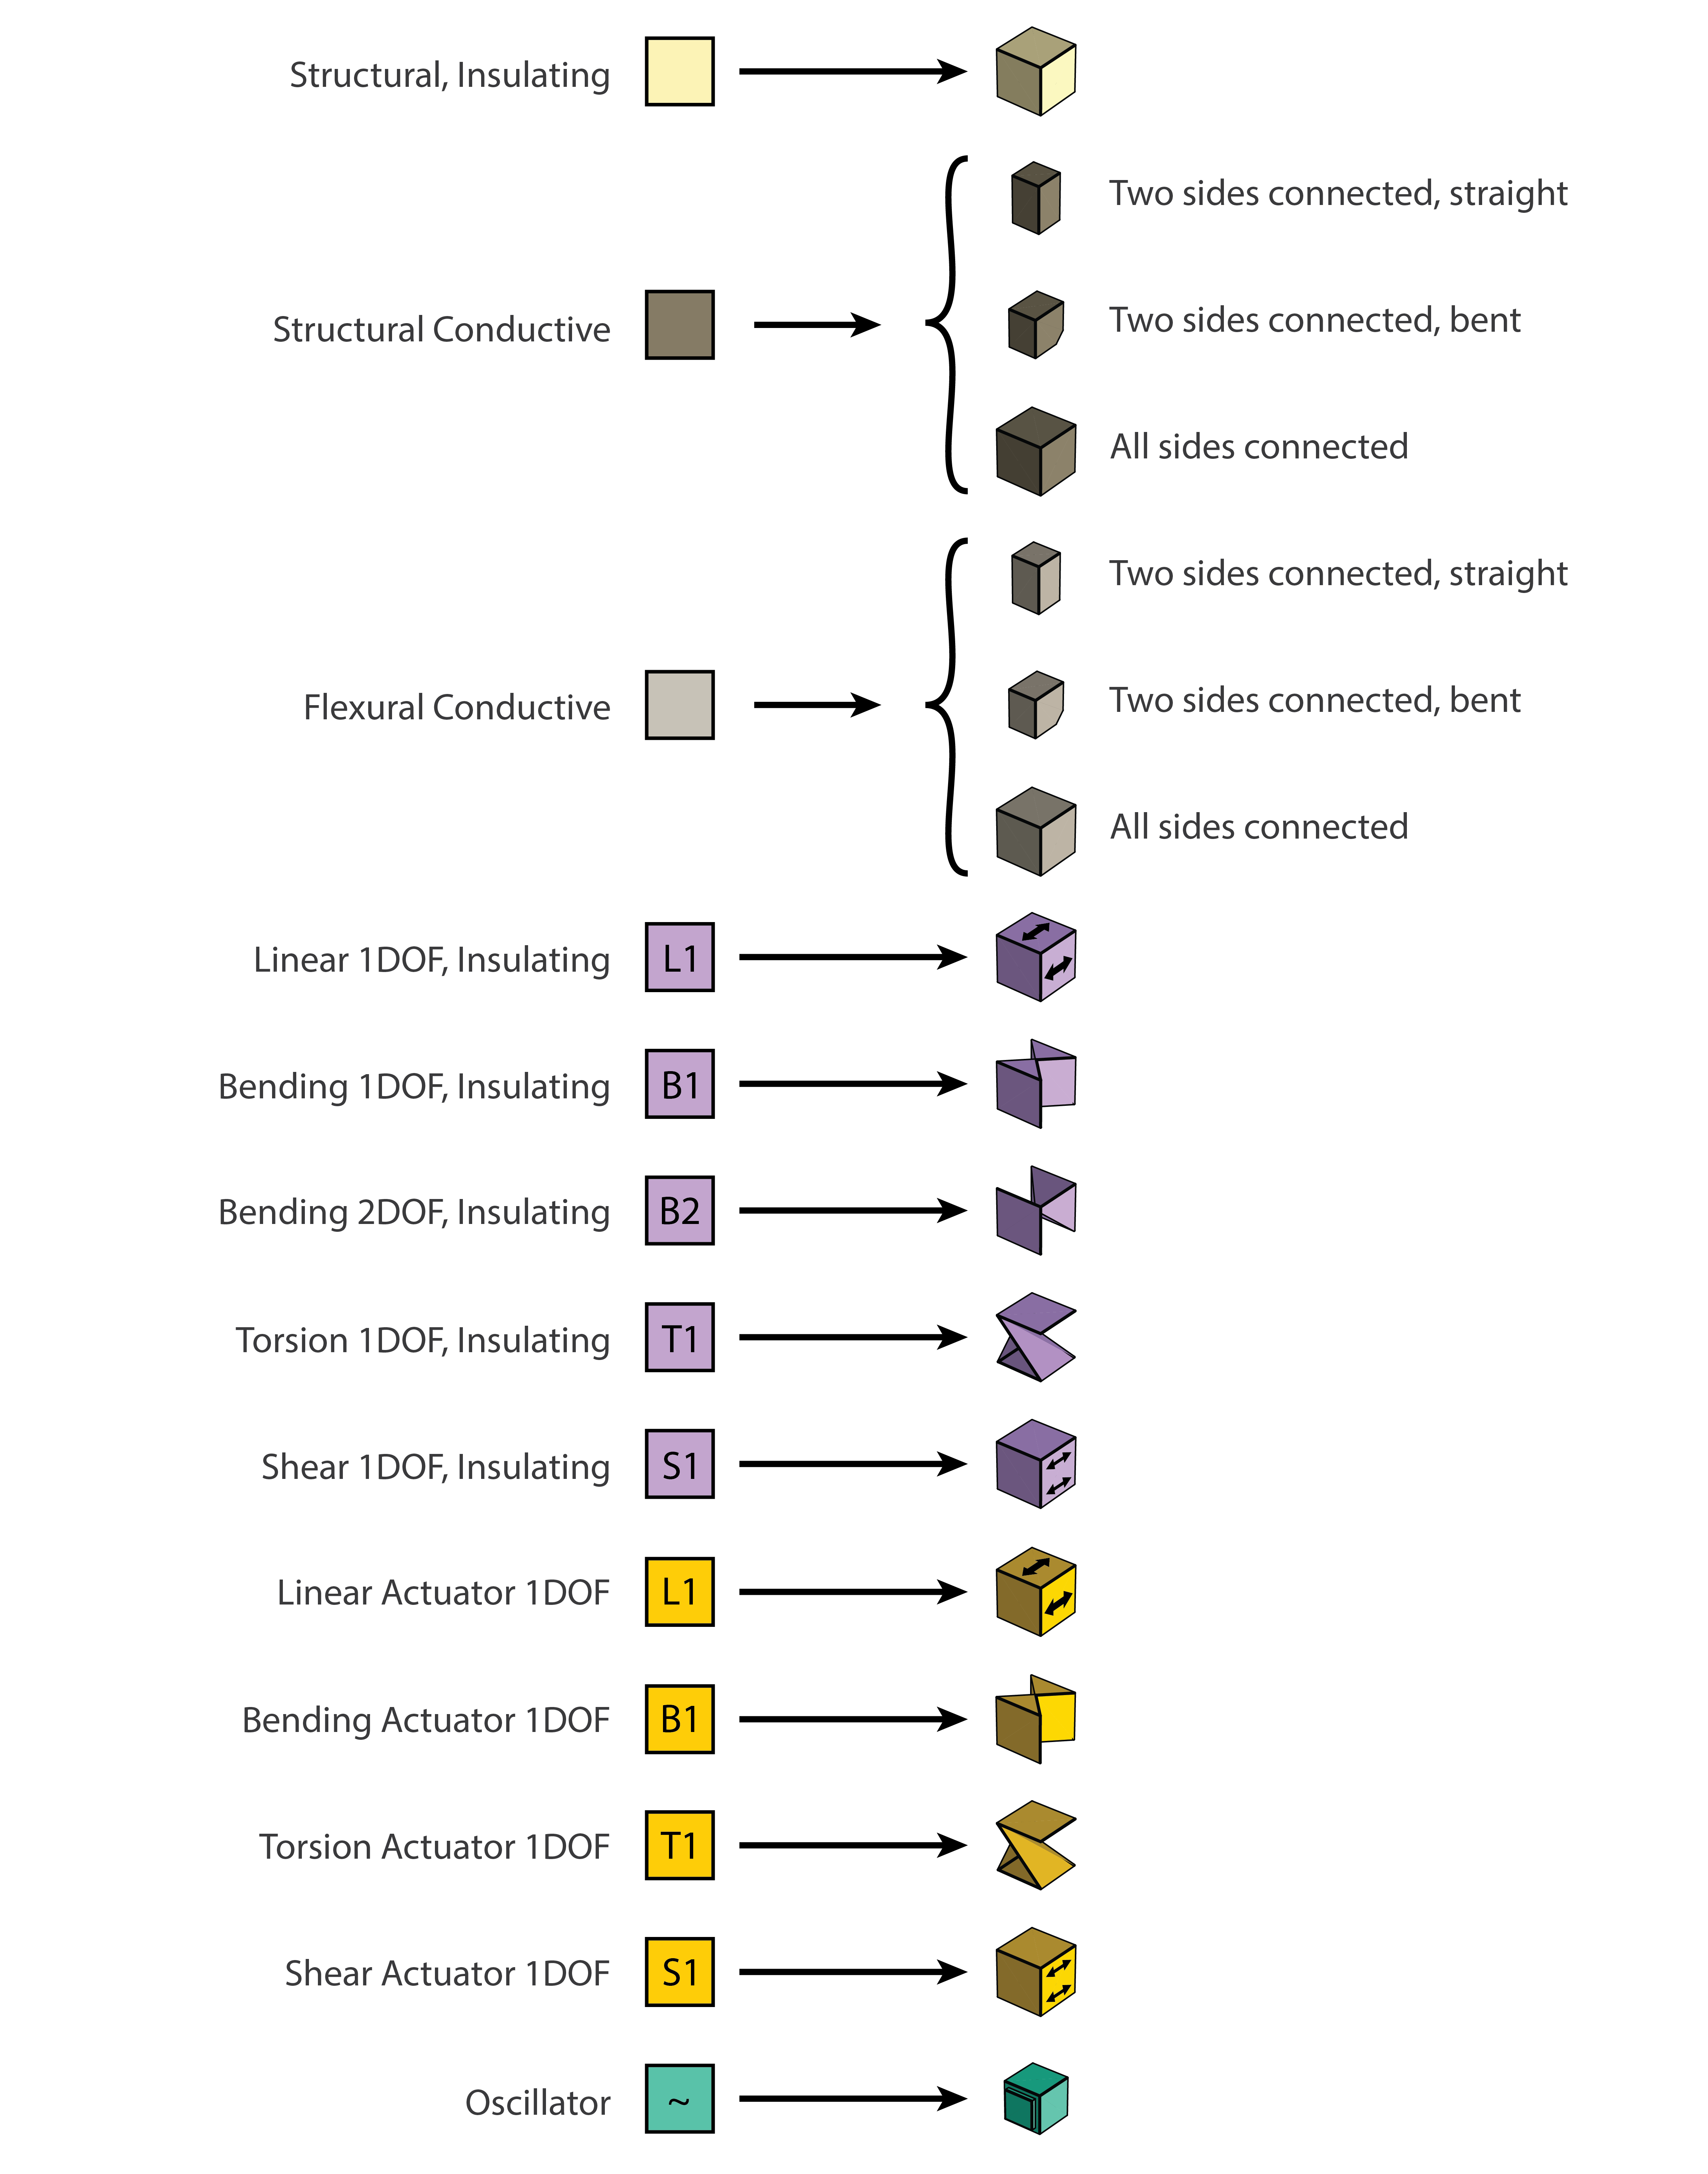
\includegraphics[width=\linewidth]{cellMeshes.png}
  \caption{Meshes and textures used to represent different material types and convey the orientation of cell anisotropy.}
  \label{fig:cellMeshes}
\end{figure}

\section{GUI}

AMOEBA borrows most of its GUI from DMDesign (Chapter \ref{chap:CAD}), with a few exceptions.  A cell rotation interface (Figure \ref{fig:rotationGUI}) allows users to rotate cells in 3D, so anisotropic cells may be oriented in any direction.  Absolute cell orientations are saved as JSON when the assembly is saved.  A 3D selection tool allows users to select large rectangular regions of space to fill with material, cut away material, and clone or mirror an existing structure into another region (Figure \ref{fig:selectiontoolGUI}).\\

\begin{figure}
  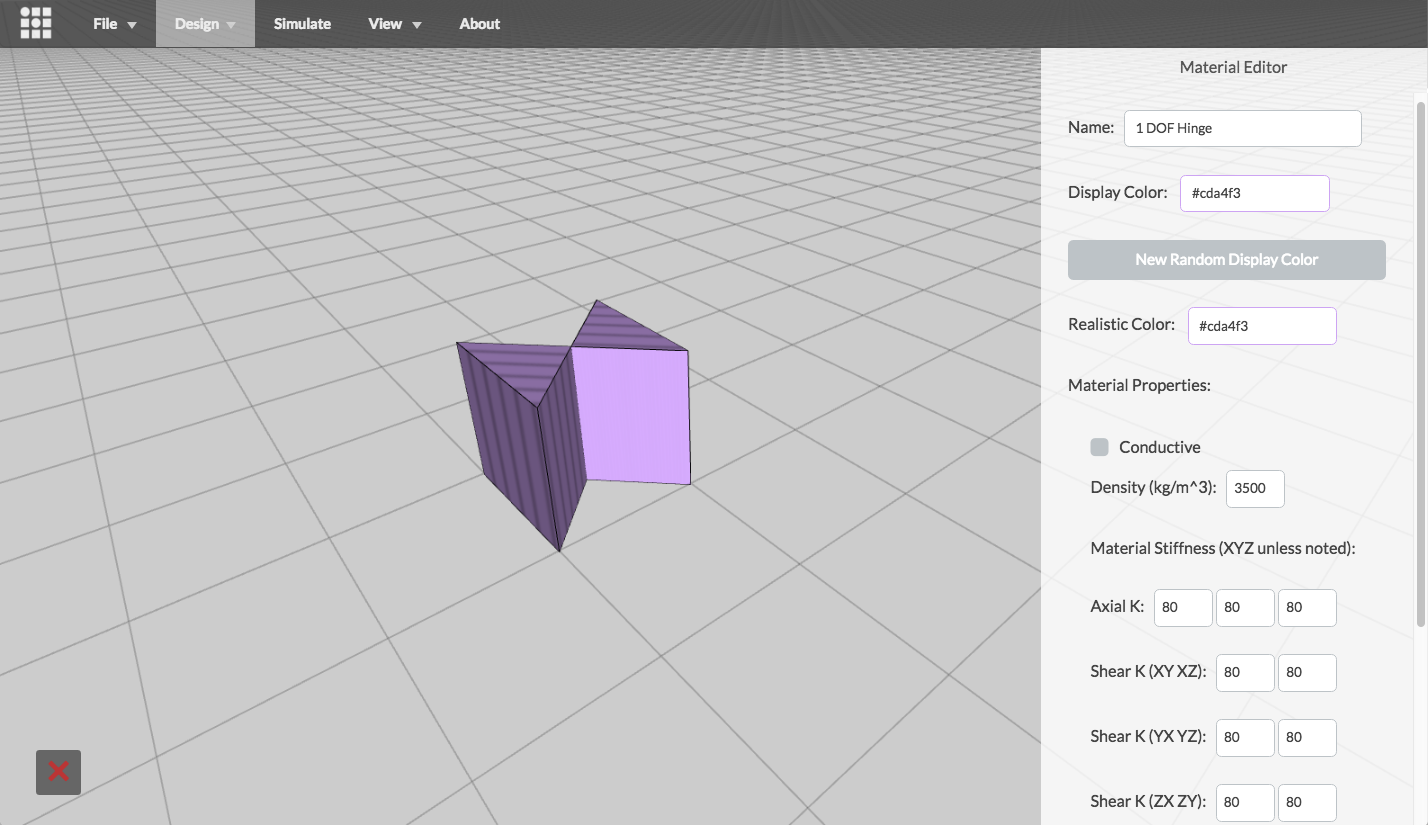
\includegraphics[width=\linewidth]{materialEditor.png}
  \caption{Material editor interface for a 1DOF bending flexure.  All 15 stiffness and damping constants may be edited, along with density and conductivity.}
  \label{fig:materialEditor}
\end{figure}

Anisotropic cells in AMOEBA are represented graphically with special meshes, illustrated in Figure \ref{fig:cellMeshes}.  Some cells (e.g. the straight and bent conducting cells) appear to occupy a smaller volume than other cells, but this is meant only as a visualization of their properties.  All cells fill the same volume and are joined mechanically with six face-connected neighbors.  Isotropic and anisotropic materials may be edited or defined through the material editor interface (Figure \ref{fig:materialEditor}).\\

\section{GPU Programming}

%JavaScript is loosely typed and therefore not an especially fast language out of the box.  Storing large datasets in typed arrays helps to speed up array operations and access at runtime \cite{Network}.  Most modern web browsers support Just In Time (JIT) compilation of JavaScript code, which helps make it more competitive with compiled languages.    Still, it tends to run slower than native C++.\\

\begin{figure}
  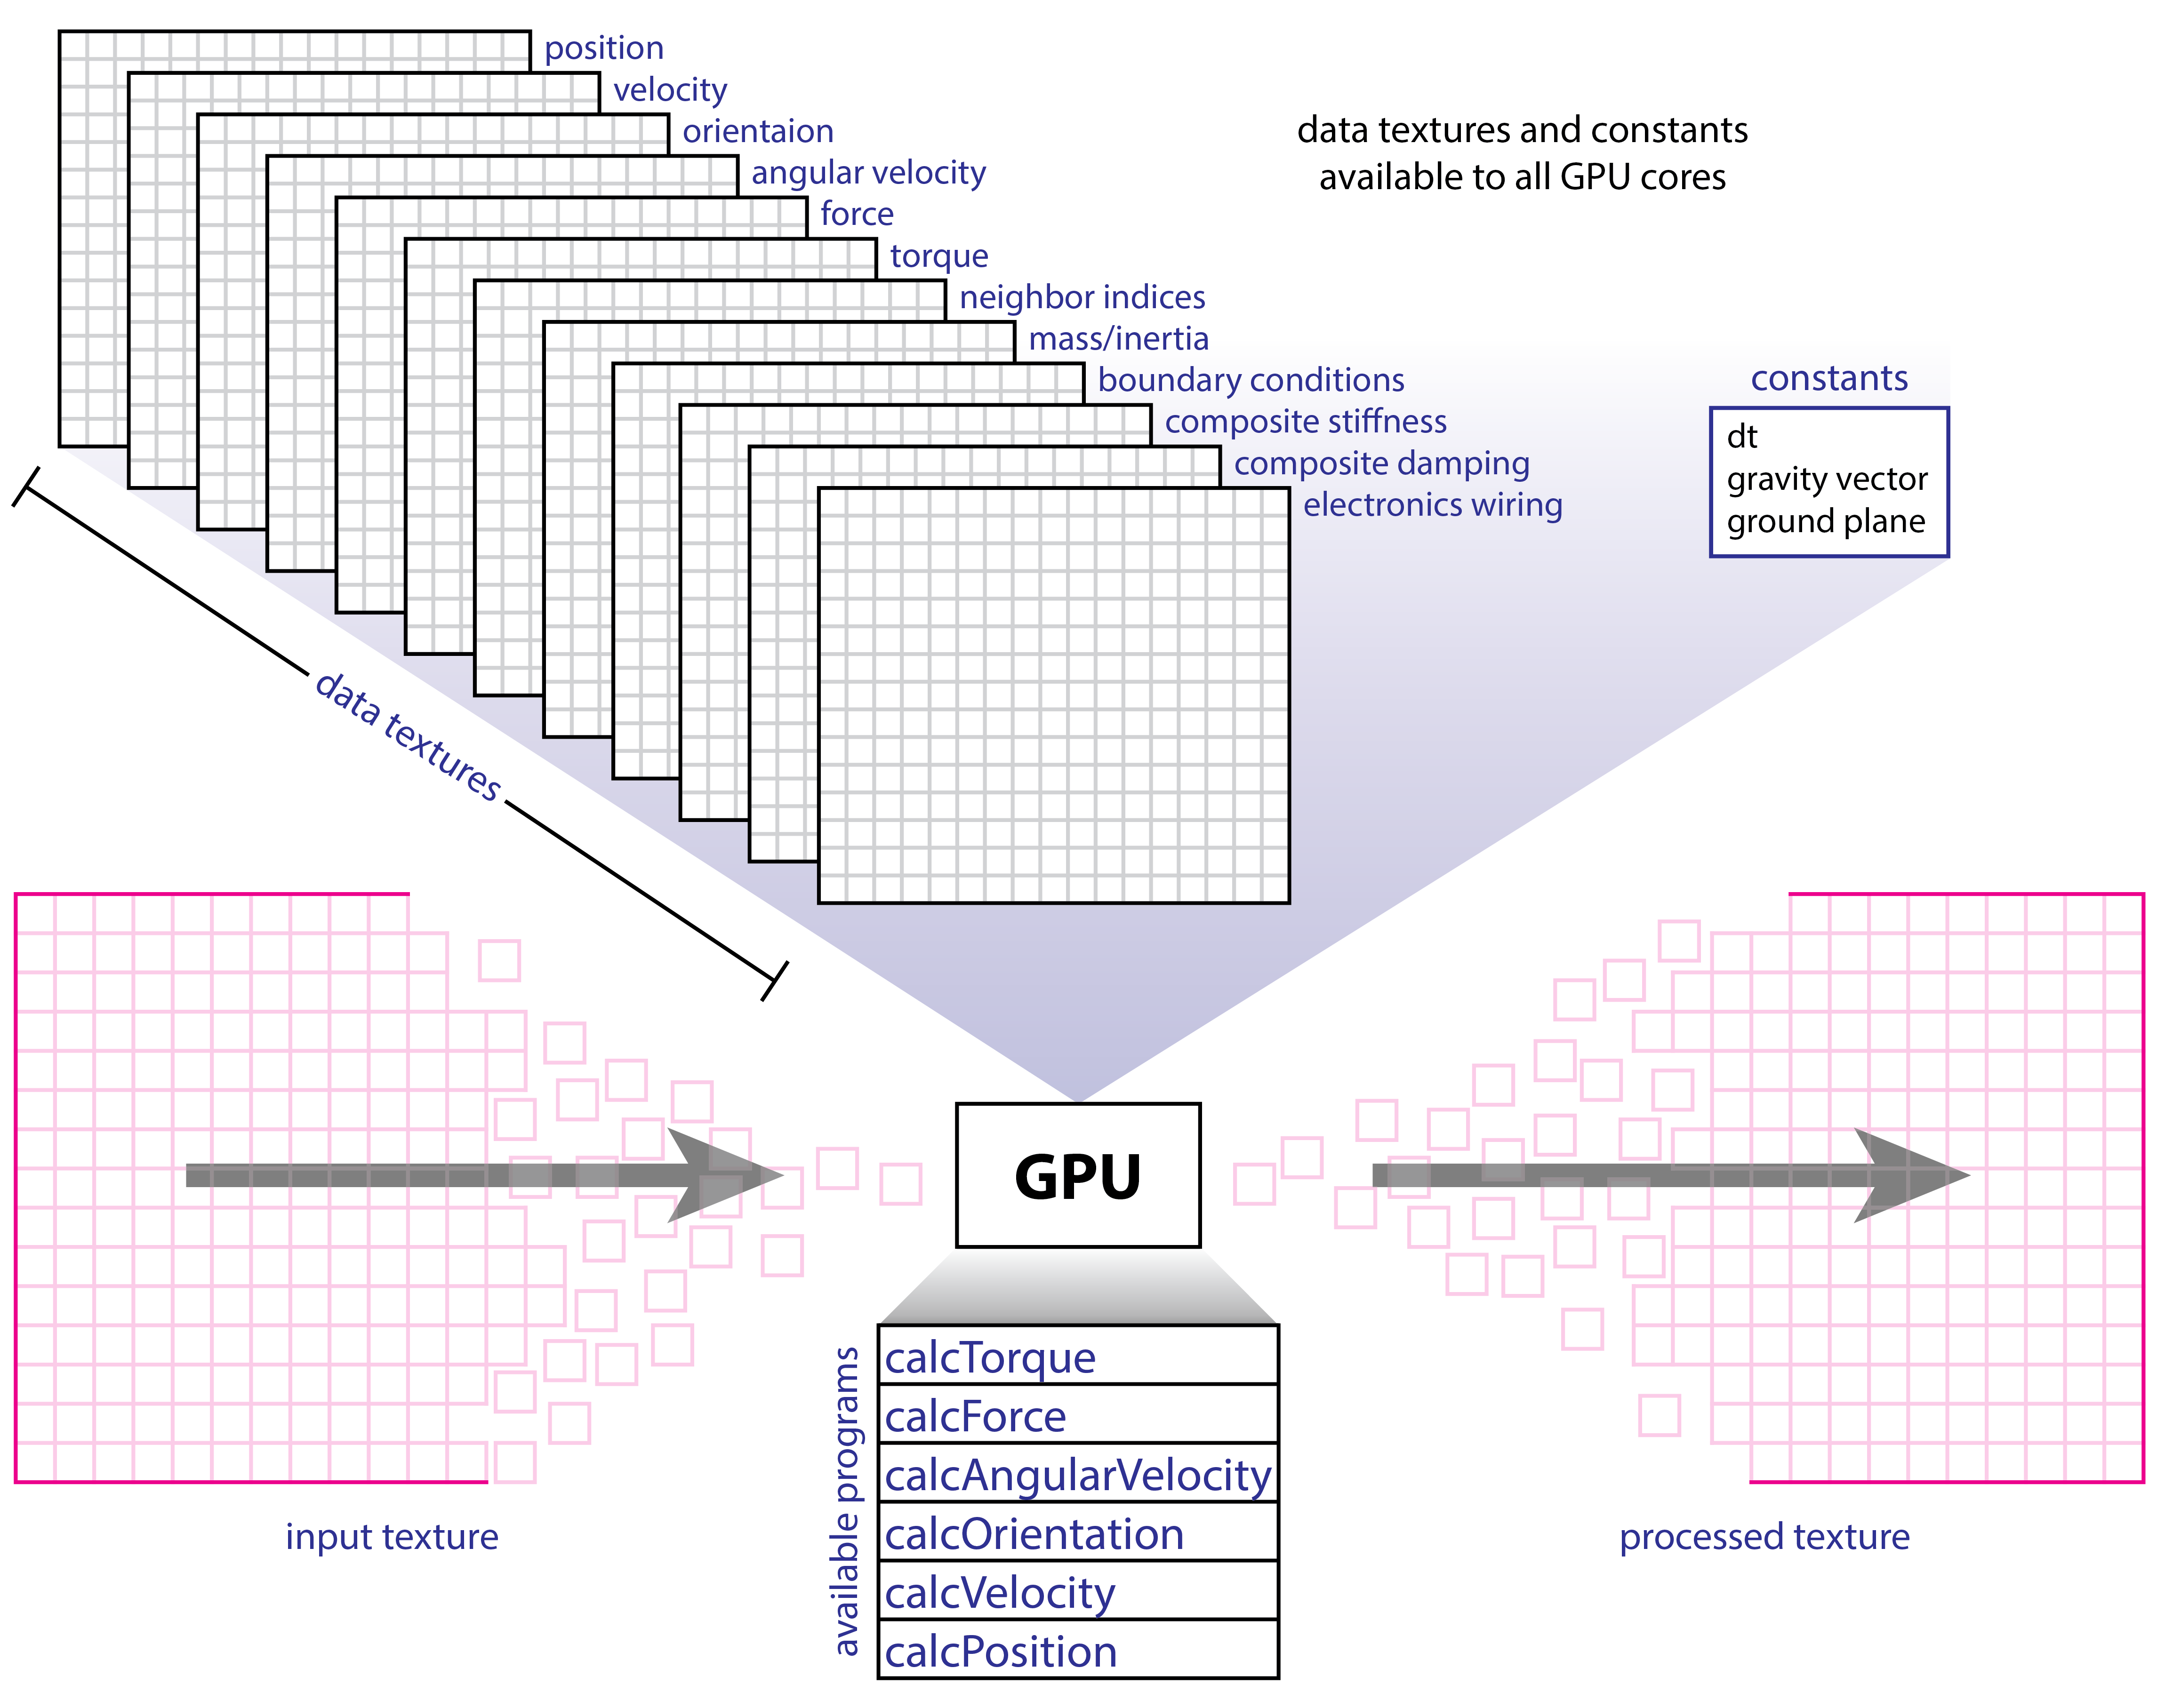
\includegraphics[width=\linewidth]{gpuprogramming.png}
  \caption{Schematic diagram of GPU programming in AMOEBA.  2D data textures store the current state of the cells, lookup tables for neighboring indices, and precomputed composite stiffness and damping constants.  These data textures as well as some global constants are passed into the GPU and are available to all cores.  An input texture buffer is sent into the GPU, split up into RGBA pixels, and used to store the output state from each core.  Several pre-compiled programs are available to the GPU, and are called sequentially during each time step of the simulation (with the exception of PackFloatToBytes, a program used to convert a Float32 texture to a uInt8 texture so that position and orientation can be extracted from the GPU for render).}
  \label{fig:gpuprogramming}
\end{figure}

During the development of AMOEBA, typed arrays \cite{Network} were not performant for assemblies larger than $\sim$30 cells (100 time steps forward per render), so I began running the bulk of the mathematical calculations on the GPU.  Figure \ref{fig:gpuprogramming} shows a schematic representation of the GPU programming.\\

At the moment of writing this, mathematical programming on the GPU through the WebGL API is a bit of a hack.  Data is passed in and out of the GPU cores as 2D arrays - RGBA image textures that would normally be used for rendering purposes.  WebGL currently supports reading and writing Int8/16/32, uInt8/16/32 and Float32 textures.  GPU programs are precompiled as \textit{fragment shaders}, processes that are executed by a single core of the GPU to create a single pixel of output texture data.  Each GPU core may access a number of input data textures but may only output one RGBA pixel to an output texture buffer.  During the execution of a fragment shader program, a complete output texture is calculated by the available GPU cores in a highly parallel, pixel-wise process.  A concise reference for the WebGL API is provided by the Khronos Group \cite{Group}.\\

In AMOEBA, cell state and precomputed constants are stored in several data textures (Figure \ref{fig:gpuprogramming}), and the next state of a given cell is evaluated in a single core of the GPU.  It is not possible to fit all necessary updated state variables (position, velocity, orientation, and angular velocity, all in 3D) in a single RGBA pixel.  This means that calculations for a single time step of the physics engine must be split into several, sequential fragment shader programs (Figure \ref{fig:gpuprogramming}).\\

After moving the simulation forward by some number of time steps, position and orientation information is passed out of the GPU to the main thread for a render call.  Unfortunately, at this time only uInt8 textures may be transferred from the GPU to the CPU.  An additional fragment shader program called ``PackToBytes'' converts the Float32 arrays storing position and orientation into uInt8 arrays, where each float in the original array is converted to four uInt8's.  The process of transferring data from the GPU to the CPU is expensive, and in the fullness of time, could be avoided completely.  AMOEBA is still very much under development and is not ready for these types of low level optimizations yet, but it is something to keep in mind in the following months.\\

Computing in the GPU speeds up the code significantly, but also creates some hardware dependencies that would not have otherwise been present.  For example, some GPUs have a hard limit of 8 textures that can be loaded into memory at a time.  In case of compatibility issues, a backup typed array implementation may be used at the expense of performance.

\section{Other Performance Speedups}

Additional speedups in mathematical operations increase runtime speed of the code.  As demonstrated in Chapter \ref{chap:functionSim}, the math behind the mechanical modeling involves liberal use of quaternions.  An efficient method of applying quaternions to vectors is given below:
\[ t = 2 \left[ \begin{array}{ccc}
q_x\\
q_y\\
q_z
 \end{array} \right] \times v\]
\[ v_{rotated} = v + q_wt +  \left[ \begin{array}{ccc}
q_x\\
q_y\\
q_z
 \end{array} \right] \times t\]
 
 This method uses fewer floating point operations than the standard Hamilton product from equation \ref{eq:hamiltonprod} \cite{Reinalter}.

\section{Instability}

\begin{figure}
  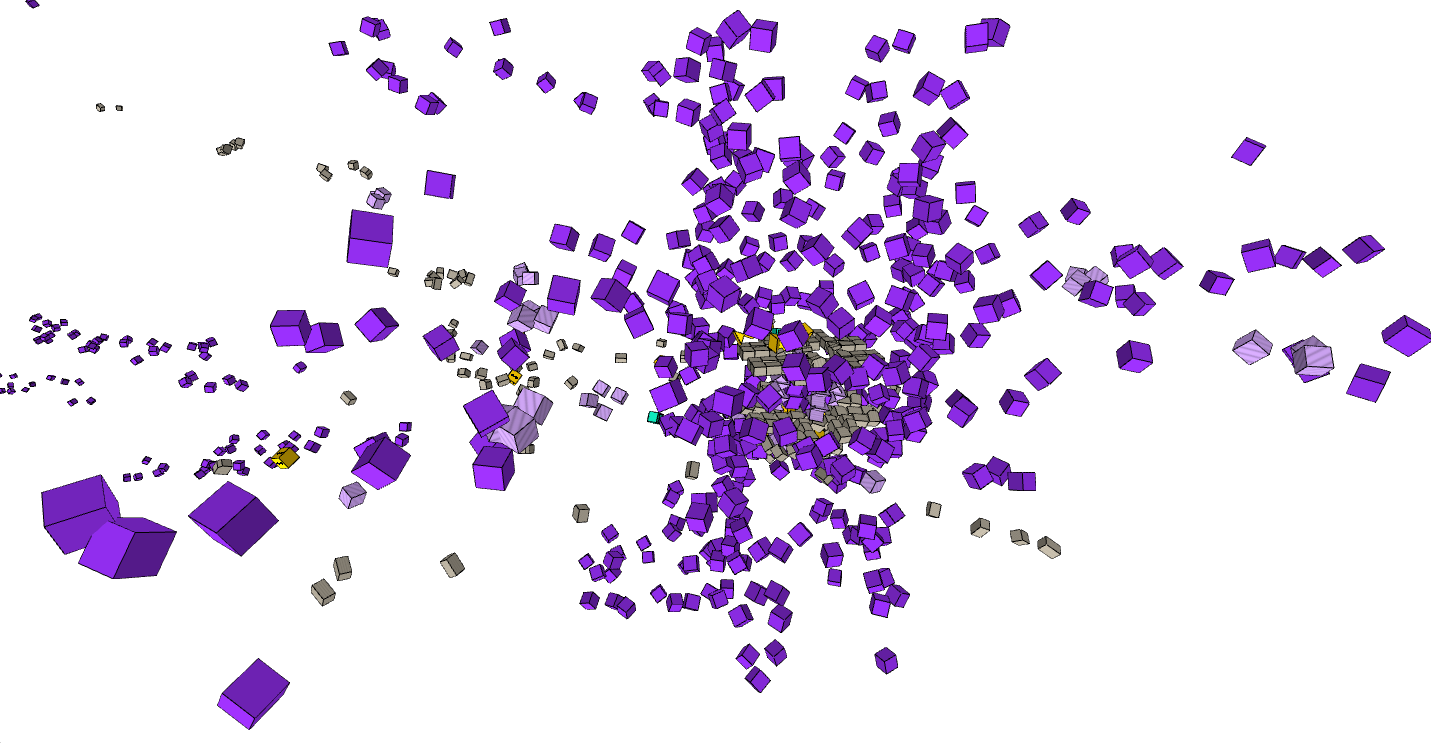
\includegraphics[width=\linewidth]{instability.png}
  \caption{In its current state, AMOEBA is suffering from instability originating in bugs in the simulation code.}
  \label{fig:instability}
\end{figure}

In its current state, AMOEBA is suffering from issues of instability related to bugs in the simulation code.  Additionally, rotational damping has not yet been implemented and its absence tends to throw the system unstable, especially in large, dense assemblies.  This instability tends to look like an explosion (Figure \ref{fig:instability}); as spring systems go unstable they result in massive displacements.  I expect this instability to be resolved in the coming months.

\section{Examples}

\begin{figure}
  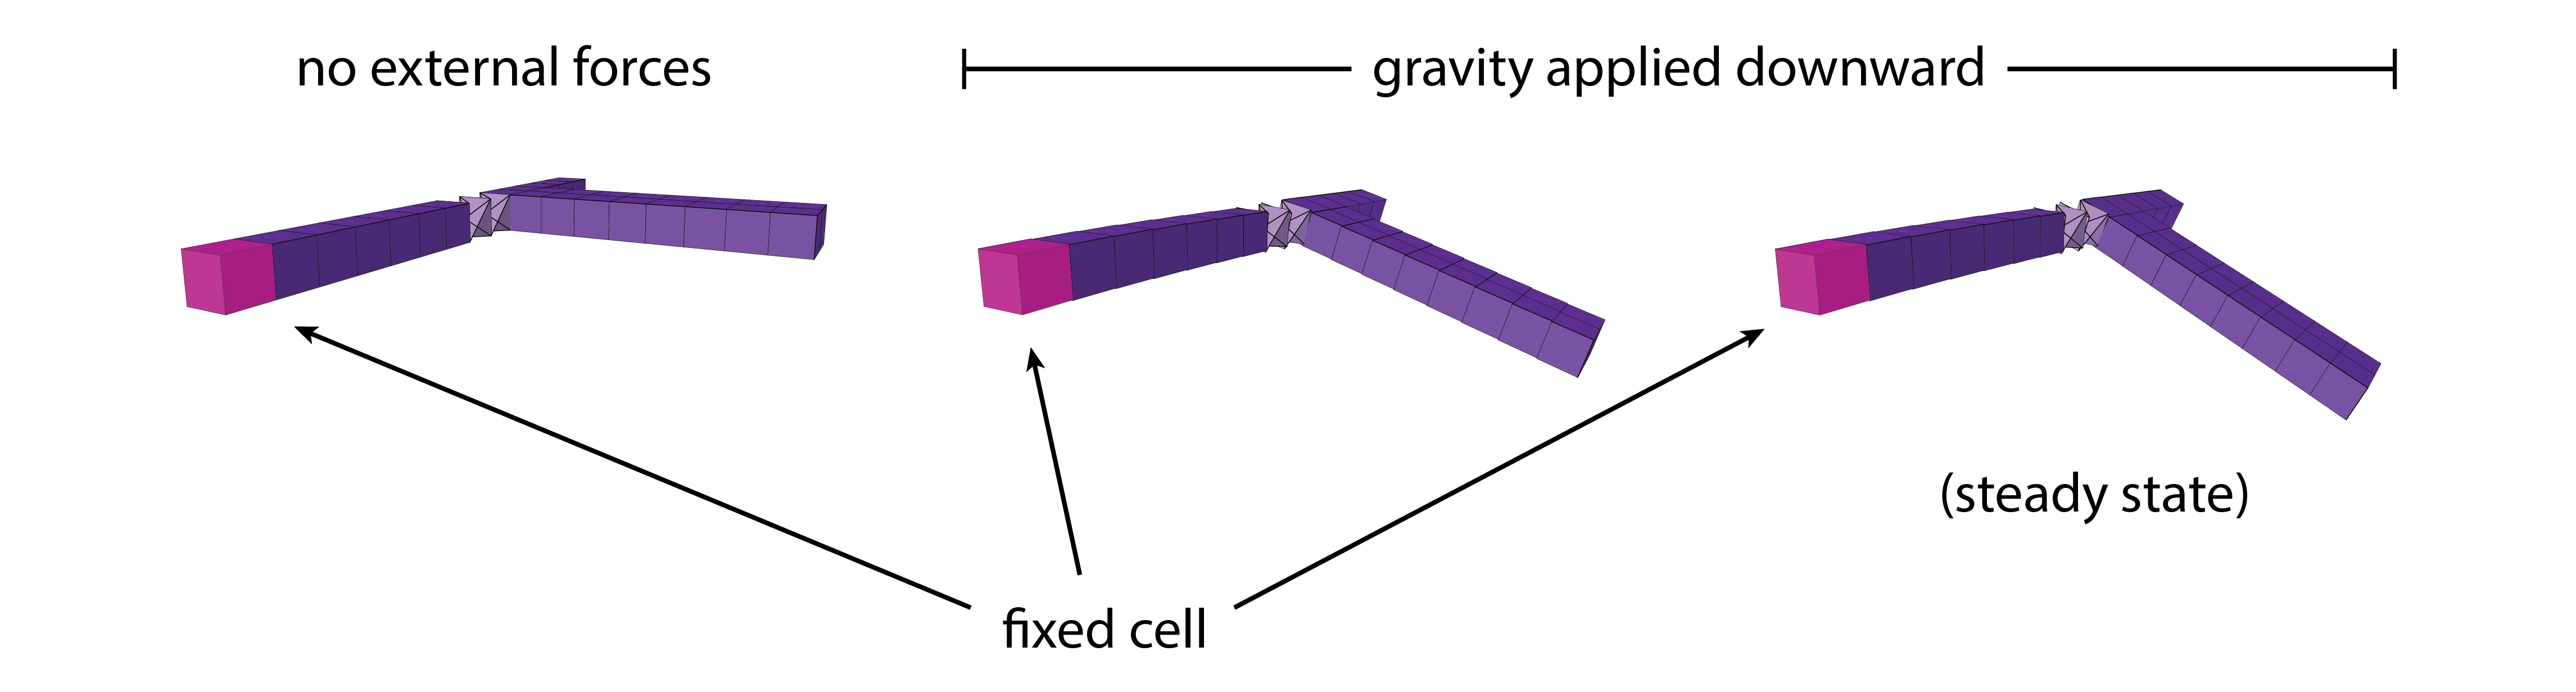
\includegraphics[width=\linewidth]{TorsionSim.png}
  \caption{Simulation of a torsional flexure under a downward force from gravity shows appropriate anisotropic behavior.  Purple are stiff cells, light purple is torsional flexures.  Pink cell is fixed.}
  \label{fig:TorsionSim}
\end{figure}

Due to instability, only certain configurations of parts are currently happy in AMOEBA.  One example is a torsional flexure shown in Figure \ref{fig:TorsionSim}.  An older version of the AMOEBA engine lacked a complete model of torsional and bending stiffness, but tended to be much more stable than the current state of development.  Several examples of simple robotic elements were constructed within this older version of the physics engine (Figures \ref{fig:beambending} through \ref{fig:undulating}).

\begin{figure}
  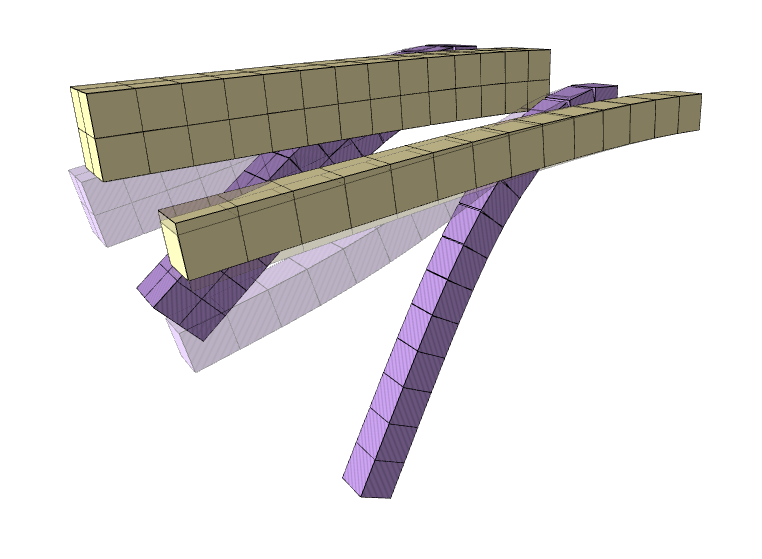
\includegraphics[width=\linewidth]{beambending.png}
  \caption{Beam bending simulation sets one end fixed and allows the rest to deform under gravity.  Both material types shown are isotropic: white material is stiffer than purple.}
  \label{fig:beambending}
\end{figure}

\begin{figure}
  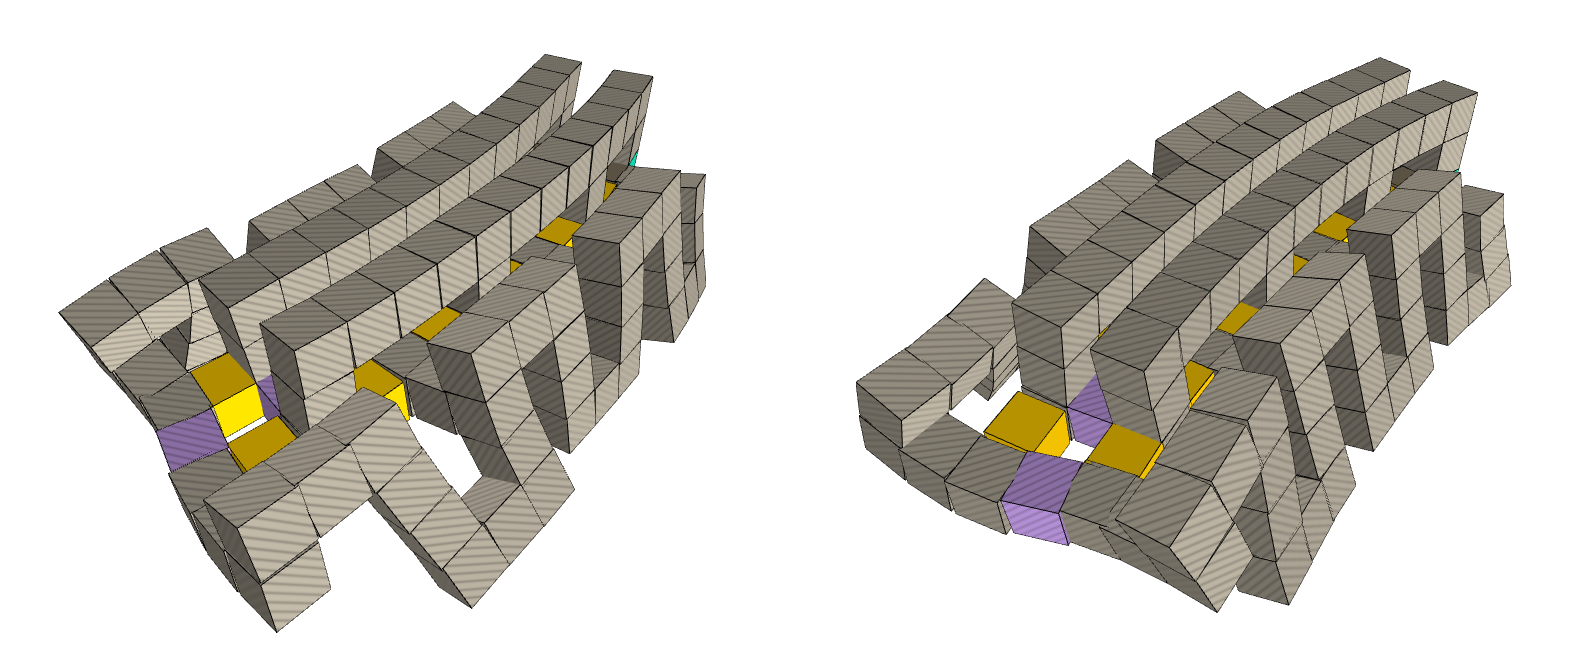
\includegraphics[width=\linewidth]{bendy.png}
  \caption{A bending structure made from two stacks of linear actuators driven out of phase from each other.}
  \label{fig:bendy}
\end{figure}

\begin{figure}
  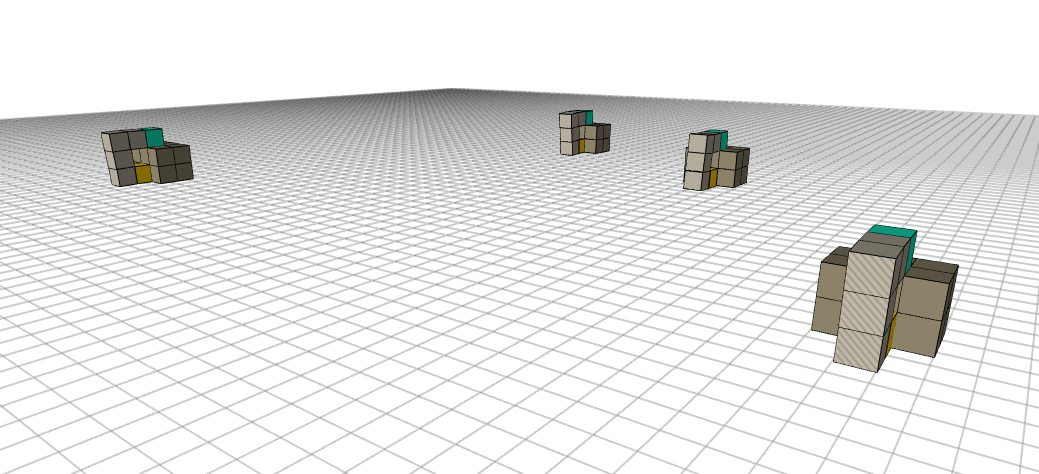
\includegraphics[width=\linewidth]{locomotionsimple.png}
  \caption{Simple locomotion demonstration shows four simple robots, each with a single linear actuator and oscillator.  Differences in speed are due to different oscillator waveforms driving each robot's circuit.  From left to right: sine, square, saw, triangle.}
  \label{fig:locomotionsimple}
\end{figure}

\begin{figure}
  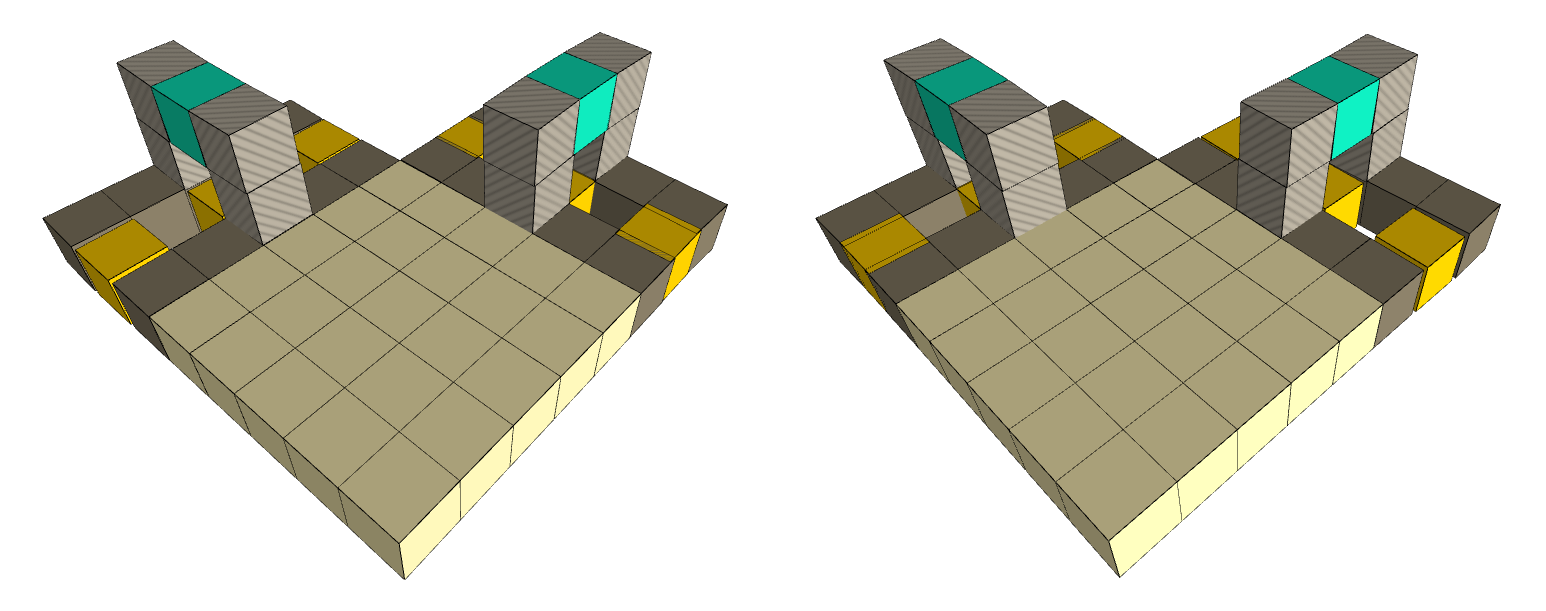
\includegraphics[width=\linewidth]{xystage.png}
  \caption{XY stage driven in a circular motion by two stacks of linear actuators a quarter cycle out of phase from each other.}
  \label{fig:xystage}
\end{figure}

\begin{figure}
  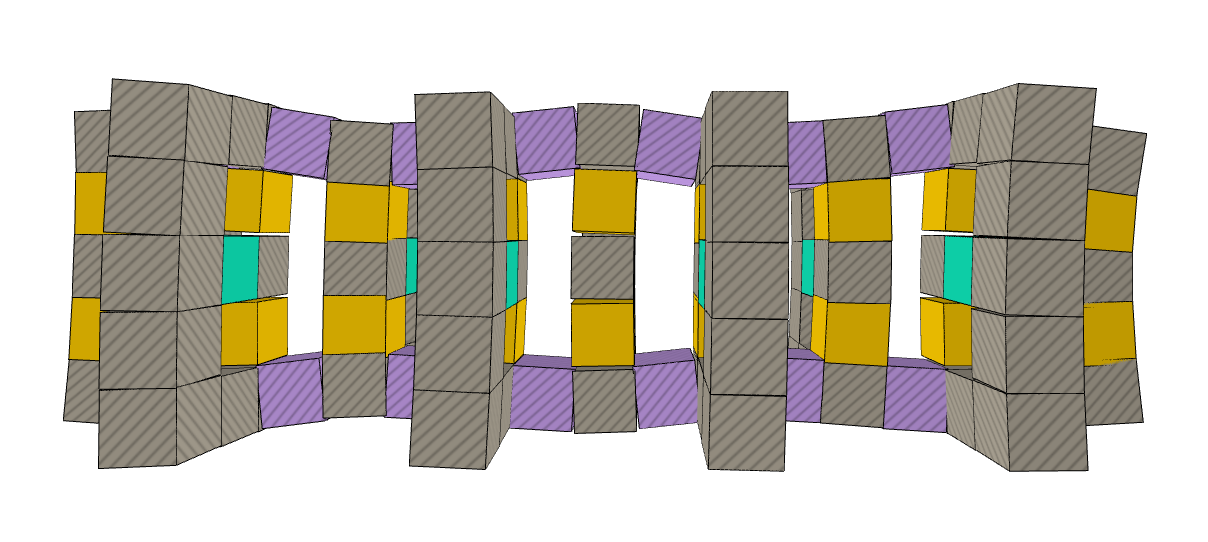
\includegraphics[width=\linewidth]{undulating.png}
  \caption{Undulating structure uses several stacks of linear actuators driven a third of a cycle out of phase from each other to create a sinusoidal motion up its spine.}
  \label{fig:undulating}
\end{figure}
